\documentclass{suribt}
\def\mbf#1{\mbox{\boldmath $#1$}} 
\def\rup#1{{^#1}\hspace{-0.5mm}}
%\documentclass[oneside]{suribt}% 本文が * ページ以下のときに (掲示に注意)
\usepackage{amsmath}
\usepackage[dvips]{graphicx}
\usepackage{cite}
%数式用の追加パッケージ
\usepackage{amsmath}
\usepackage{bm}
\renewcommand{\figurename}{Fig.}

%\title{CLデータに基づく微小摺動制御法を用いたデスクトップ型NC工作機械}
\title{\huge Xtion Pro Liveカメラを用いた\\複数移動ロボットのビジュアルフィードバック制御の基礎実験計}
%\titlewidth{}% タイトル幅 (指定するときは単位つきで)
\author{三木 康平}
\eauthor{Hiroaki kurisu}% Copyright 表示で使われる
\studentid{F112026}
\supervisor{永田寅臣 教授}% 1 つ引数をとる (役職まで含めて書く)
%\supervisor{指導教員名 役職 \and 指導教員名 役職}% 複数教員の場合,\and でつなげる
\handin{2016}{03}% 提出月. 2 つ (年, 月) 引数をとる
%\keywords{キーワード1, キーワード2} % 概要の下に表示される
\begin{document}
\maketitle %%%%%%%%%%%%%%%%%%% タイトル %%%%
\frontmatter %ここから前文
\begin{abstract}%%%%%%%%%%%%% 概要 %%%%%%%%%%%%%%%%%%%%%


%%%%%%%%%%%%%%%%%%%%%%%%%%%%%%%%%%%%%%%%%%%%%%%%%%%%%%%%%


\end{abstract}
\tableofcontents%%%%%%%%%%%%% 目次 %%%%%%%%
\mainmatter% ここから本文 %%% 本文 %%%%%%%%
%%%%%%%%%%%%%%%%%%%%%%%%%%%%%%%%%%%%%%%%%%%%%%%%%%%%%%%%%%%%%%%%
%%%%%%%%%%%%%%%%%%%%%%%%%%%%%%%%%%%%%%%%%%%%%%%%%%%%%%%%%%%%%%%%
%%%%%%%%%%%%										%%%%%%%%%%%%
%%%%%%%%%%%%				第1章					%%%%%%%%%%%%
%%%%%%%%%%%%										%%%%%%%%%%%%
%%%%%%%%%%%%%%%%%%%%%%%%%%%%%%%%%%%%%%%%%%%%%%%%%%%%%%%%%%%%%%%%
%%%%%%%%%%%%%%%%%%%%%%%%%%%%%%%%%%%%%%%%%%%%%%%%%%%%%%%%%%%%%%%%
%%%%%%%%%%%%%%%%%%%%%%%%%%%%%%%%%%%%%%%%%%%
\chapter{緒言}
%%%%%%%%%%%%%%%%%%%%%%%%%%%%%%%%%%%%%%%%%%%
近年, 消費者嗜好の多様化により, 商品生産方式が少品種大量生産から変種変量生産へと変わってきている. それに応じて, ロボットも単一工程に特化した産業用ロボットから, 人のように状況判断を行い, 幅のある業務をこなすことができるような汎用機械としてのロボットへと, ニーズが変化してきている~\cite{Iziri-2019}. このニーズに応えるため, さまざまな画像処理を自動で行うカメラや, ベルトコンベア上の製品を自動で仕分けするロボットビジョンなどが販売されているが, カメラや光源の位置が限られる狭い空間内において, 対象物を画像処理により検出し移動させるシステムの実現は難しい. そこで, 研究室では狭い空間内での正確な物体の検出および移動を最終的な目標としたシステムの研究を行っている. 本研究では, 現在取り組んでいるシステムの進捗について報告する. 

課題に取り組むに当たって, まず開けた空間内に平面に置かれた物体を画像認識と人工知能技術(AI)を用いた角度推定により, 対象物の角度を依らず, 正確にピック&プレースを行うロボットシステムを開発した. この手法では, 画像内に写るオブジェクトの角度をAIで推定し, アームでPickingを行う. 具体的には, 対象物をカメラにより撮影し, まず画像認識により対象物の重心位置を計算し, その位置までアームを移動させる. その後, 角度推定用にAlexNetを基に転移学習したネットワークがその角度を推定する. そして, アームに付属するエンドエフェクタを推定角度だけ回転させ, 対象物をPickingする. 

%%%%%%%%%%%%%%%%%%%%%%%%%%%%%%%%%%%%%%%%%%%%%%%%%%%%%%%%%%%%%%%%
%%%%%%%%%%%%%%%%%%%%%%%%%%%%%%%%%%%%%%%%%%%%%%%%%%%%%%%%%%%%%%%%
%%%%%%%%%%%%										%%%%%%%%%%%%
%%%%%%%%%%%%				第2章					%%%%%%%%%%%%
%%%%%%%%%%%%										%%%%%%%%%%%%
%%%%%%%%%%%%%%%%%%%%%%%%%%%%%%%%%%%%%%%%%%%%%%%%%%%%%%%%%%%%%%%%
%%%%%%%%%%%%%%%%%%%%%%%%%%%%%%%%%%%%%%%%%%%%%%%%%%%%%%%%%%%%%%%%
%%%%%%%%%%%%%%%%%%%%%%%%%%%%%%%%%%%%%%%%%%%%%%%%%%%%%%%%%%%%%%%%%%%%%%%%%%%%%
\chapter{運動学}
%%%%%%%%%%%%%%%%%%%%%%%%%%%%%%%%%%%%%%%%%%%%%%%%%%%%%%%%%%%%%%%%%%%%%%%%%%%%%
ロボットアームの手先を目的の位置に移動させたいとき, 各関節角度と関節間の長さ現在の手先位置が分かっていれば, 運動学を用いて必要な姿勢を計算することが出来る. 運動学とは, ロボットアームの関節角度や関節間の長さと手先位置・姿勢の関係を数式で表したものであり, 各関節角度から手先位置・姿勢を求めることを順運動学, 手先位置・姿勢から各関節角度を求めることを逆運動学という. 
また, ロボットアームは各関節ごとに座標系(関節座標系)を設定することができ, この座標系と台座部に設定した基準座標系は運動学に用いることで互いに変換することができる.

%%%%%%%%%%%%%%%%%%%%%%%%%%%%%%%%%%%%
\section{順運動学}
%%%%%%%%%%%%%%%%%%%%%%%%%%%%%%%%%%%%
順運動学とは, ロボットアームの各関節角度の変位(回転・並進)から手先位置・姿勢を求めることであり, すなわち手先位置の関節座標系から基準座標系への変換ということができる. また, 順運動学は各関節の回転と並進の要素を持つ. 

%%%%%%%%%%%%%%%%%%%%%%%%%%%%%%%%%%%%
\subsection{計算方法}
%%%%%%%%%%%%%%%%%%%%%%%%%%%%%%%%%%%%
ここでは関節座標の手先位置を基準座標系に変換する方法について示す. まず簡単のために図\ref{fig:translation}のような系について考える.
%------------
%Figure translation
%------------
\begin{figure}[ht]
 \begin{center}
  \includegraphics[width=60mm,clip]{./figure/translation.eps}
  \caption{Polishing scene using a conventional industrial robot with a servo spindle.}
  \label{fig:translation}
 \end{center}
\end{figure}

移動後の原点$O'(x_0', y_0', z_0')$は, 移動前の原点$O(x_0, y_0, z_0)$から見ると次のように表される.
%------------
%数式 並進移動_1
%------------
\begin{eqnarray*}
	x_0' = x_0 + x_1 \\
	y_0' = y_0 + y_1 \\
	z_0' = z_0 + z_1
\end{eqnarray*}

上式をベクトル${\bm r}$を用いて表すと, 以下のようになる.
%------------
%数式 並進移動_ベクトル
%------------
\begin{equation}
	\label{O-O'translation}
	O' = O + {\bm r}
\end{equation}

関節座標系から基準座標系への変換を行うには、並進移動だけでなく回転移動についても考える必要がある. そこで図\ref{fig:1rink}のような簡単な系の回転移動について考える.
%------------
%Figure 1rink
%------------
\begin{figure}[ht]
 \begin{center}
  \includegraphics[width=60mm,clip]{./figure/1rink.eps}
  \caption{Polishing scene using a conventional industrial robot with a servo spindle.}
  \label{fig:1rink}
 \end{center}
\end{figure}

 まずベクトル${\bm P}(x_1, y_1, z_1)$は, 各軸方向の単位ベクトル(${\bm i}, {\bm j}, {\bm k}$)を用いて次のように表される.
%------------
%Pベクトル
%------------
\begin{equation}
	\label{Pvector}
	{\bm P} = x_1{\bm i} + y_1{\bm j} + z_1{\bm k}
\end{equation}

次に, Z軸を基準としてベクトル${\bm P}$を含むX-Y平面を$\theta$だけ回転した座標系を新しく$X', Y', Z'$座標系とすると, その座標系におけるとすると, ベクトル${\bm P'}(x_2, y_2, z_2)$は単位ベクトル${\bm i'}, {\bm j'}, {\bm k'}$を用いて次のように表される.
%------------
%P'ベクトル
%------------
\begin{equation}
	\label{P'vector}
	{\bm P'} = x_2{\bm i'} + y_2{\bm j'} + z_2{\bm k'}
\end{equation}

ここで, 単位ベクトル単位ベクトル${\bm i'}, {\bm j'}, {\bm k'}$は回転前の座標系から見ると

%------------
%単位ベクトルの回転行列
%------------
\begin{equation}
	\label{RotationMatrix}
	\left[
		\begin{array}{c}
			{\bm i'} \\
			{\bm j'} \\
			{\bm k'}
		\end{array}
	\right]
	=
	\left[
		\begin{array}{ccc}
			\cos \theta & \sin \theta & 0 \\
			-\sin \theta & \cos \theta & 0 \\
			0                & 0                 & 0
		\end{array}
	\right]
	\left[
		\begin{array}{c}
			{\bm i} \\
			{\bm j} \\
			{\bm k}
		\end{array}
	\right]
\end{equation}

と表せる. さらに式(\ref{RotationMatrix})に式(\ref{P'vector})と式(\ref{Pvector})を代入すると

%------------
%単位ベクトルの回転行列
%------------
\begin{eqnarray*}
	\left[
		\begin{array}{c}
			x_2 \\
			y_2 \\
			z_2
		\end{array}
	\right]
	=
	\left[
		\begin{array}{ccc}
			\cos \theta & \sin \theta & 0 \\
			-\sin \theta & \cos \theta & 0 \\
			0                & 0                 & 0
		\end{array}
	\right]
	\left[
		\begin{array}{c}
			x_1 \\
			y_1 \\
			z_1
		\end{array}
	\right]
\end{eqnarray*}

さらに見通しをよくするため, 単位ベクトルを省略し以下のように表す.


%------------
%単位ベクトルの回転行列
%------------
\begin{equation}
	\label{P-P'RotationMatrix}
	{\bm P'}
	=
	\left[
		\begin{array}{ccc}
			\cos \theta & \sin \theta & 0 \\
			-\sin \theta & \cos \theta & 0 \\
			0                & 0                 & 0
		\end{array}
	\right]
	{\bm P}
\end{equation}

 すなわちZ軸を基準としたベクトルの回転移動は, 移動前後の位置移動および相対角$\theta$を用いて表すことができ, これはX軸, Y軸においても成り立つ. この式(\ref{P-P'RotationMatrix})中央の行列を回転行列といい$R$で表すこととする. 
並進移動と回転移動とを用いることにより, 図\ref{fig:ComplexTransform}に示すような一見複雑な座標系の変換も次のような式で表すことができる.

%------------
%Figure ComplexTransform
%------------
\begin{figure}[ht]
 \begin{center}
  \includegraphics[width=60mm,clip]{./figure/ComplexTransformation.eps}
  \caption{Polishing scene using a conventional industrial robot with a servo spindle.}
  \label{fig:ComplexTransform}
 \end{center}
\end{figure}

%------------
%座標変換の一般式
%------------
\begin{equation}
	^{A}{\bm P} = {^{A}{\bm R}_B}{^{B}{\bm P}} + ^{A}{\bm r}_B
\end{equation}

 ここで${^{A}{\bm R}_B}$は座標系Aから座標系Bへの回転行列である. この関係を各関節ごとに用いることで, 手先位置を基準座標系からの位置として求めることができる.

%%%%%%%%%%%%%%%%%%%%%%%%%%%%%%%%%%%%
\section{逆運動学}
%%%%%%%%%%%%%%%%%%%%%%%%%%%%%%%%%%%%
順運動学が座標変換を行うことで解が1つ求まるのに対して, 逆運動学では図\ref{fig:InverseKinematics}の場合のように手先位置が同じ位置にある場合でも各リンクの位置と姿勢にはいくつかの解が存在することや, 解自体が存在しないこともある. このような問題があるため, 一般に順運動学より逆運動学の方が問題を解くのが難しい.
%------------
%Figure Inverse kinematics
%------------
\begin{figure}[ht]
 \begin{center}
  \includegraphics[width=40mm,clip]{./figure/InverseKinematics.eps}
  \caption{Polishing scene using a conventional industrial robot with a servo spindle.}
  \label{fig:InverseKinematics}
 \end{center}
\end{figure}

%------------
%Figure 2rink
%------------
\begin{figure}[ht]
 \begin{center}
  \includegraphics[width=60mm,clip]{./figure/2rink.eps}
  \caption{Polishing scene using a conventional industrial robot with a servo spindle.}
  \label{fig:2rink}
 \end{center}
\end{figure}

逆運動学でアームの関節角度を計算する例として, 図\ref{fig:2rink}のような場合を考える. まず, 角度$\alpha$と$|{\bm {OP}}|$の関係は余弦定理を用いて次式で表される.
%------------
%数式 2リンクの手先位置_1
%------------
\begin{equation}
		\label{alpha-OPRelationship}
		\cos \alpha = \frac{L^2_1 + L^2_2 - |{\bm {OP}}|}{2 L_1 L_2}
\end{equation}

式(\ref{alpha-OPRelationship})より角度$\alpha$は$\alpha = \cos^{-1}(\cos \alpha)$と表せるので, 結果的に$\theta_2$は次式で表される.
%------------
%数式 θ2と角度αとの関係
%------------
\begin{equation}
	\theta_2 = \pi - \alpha
\end{equation}

同様に, 余弦定理を用いて角度$\beta$と$|OP|$の関係は次式で表され,
%------------
%数式 角度βと補助線OPとの関係
%------------
\[
	\cos \beta = \frac{|{\bm {OP}}|^2 + L^2_1 - L^2_2}{2 |{\bm {OP}}| L_2}
\]

$\beta = \cos^{-1}(\cos \beta)$である. 最後に角度$\gamma$は, 補助線$|{\bm OP}|$と手先位置のx座標との関係から
%------------
%数式 角度γと補助線OPとの関係
%------------
\[
	\cos \gamma = \frac{x}{|{\bm {OP}}|}
\]

であるので, $\gamma = \cos^{-1}(\cos \gamma)$ である. よって, 角度$\beta$および角度$\alpha$を用いて$\theta_1$は次式で表される.
\begin{equation}
	\theta_1 = \gamma - \beta
\end{equation}

よって, 手先位置から関節角度$\theta_1$, $theta_2$を求めることができた.

%------------
%Figure 2rink_2
%------------
\begin{figure}[ht]
 \begin{center}
  \includegraphics[width=60mm,clip]{./figure/2rink_2.eps}
  \caption{Polishing scene using a conventional industrial robot with a servo spindle.}
  \label{fig:2rink_2}
 \end{center}
\end{figure}

また別の方法として, 図\ref{fig:2rink_2}のような場合を考える. この場合, 手先位置は次式で表される.
%------------
%数式 2リンクの手先位置_2
%------------
\begin{align}
	\begin{aligned}
		\label{ForwardKinematicEquation}
		x_p = l_1 \cos \theta_1 + l_2 \cos(\theta_1 + \theta_2) \\
		y_p = l_1 \sin \theta_1 + l_2 \sin(\theta_1 + \theta_2) 
	\end{aligned}
\end{align}

式(\ref{ForwardKinematicEquation})の両辺を時間で微分し, 行列で表すと
%------------
%数式 手先位置の速度と各関節の角速度の関係
%------------
\begin{equation}
	\label{ForwardKinematicEquation_diff}
	\frac{d{\bm P}}{dt} = {\bm J}({\bm \theta})\frac{d{\bm \theta}}{dt}
\end{equation}

ここで
%------------
%数式 手先位置の速度と各関節の角速度の関係の変数
%------------
\[
{\bm P} = \left[x_p, y_p \right]^{\mathrm{T}}, {\bm \theta} = \left[\theta_1, \theta_2\right]^{\mathrm{T}}, 
{\bm J}({\theta}) = 
	\left[
		\begin{array}{cc}
			-(l_1 \sin \theta_1 + l_2 \sin(\theta_1 + \theta_2) & -l_2 \sin(\theta_1 + \theta_2) \\
			l_1 \cos \theta_1 + l_2 \cos(\theta_1 + \theta_2) & l_2 \cos(\theta_1 + \theta_2)
		\end{array}
	\right]
\]

である. 式(\ref{ForwardKinematicEquation_diff})は手先位置の速度と各関節における角速度の関係を表しており, 両辺の変換を担う行列${\bm J}$を一般にヤコビ行列という. 
さて, 逆運動学は手先位置から各関節角度を求める問題のことであったので, 式(\ref{ForwardKinematicEquation_diff})を以下のように変形する.
%------------
%数式 ヤコビ行列の逆行列
%------------
\begin{equation}
	\label{ForwardKinematicEquation_diff}
	\frac{d{\bm \theta}}{dt} = {\bm J}^{-1}\frac{d{\bm P}}{dt}
\end{equation}

しかし, ${\bm J^{-1}}$は必ずしも存在しない. ${\bm J^{-1}}$が存在しない条件は, det${\bm J^{-1}}$で求めることができ, その時の姿勢を特異姿勢もしくは特異点という. 

%%%%%%%%%%%%%%%%%%%%%%%%%%%%%%%%%%%%%%%%%%%%%%%%%%%%%%%%%%%%%%%%
%%%%%%%%%%%%%%%%%%%%%%%%%%%%%%%%%%%%%%%%%%%%%%%%%%%%%%%%%%%%%%%%
%%%%%%%%%%%%										%%%%%%%%%%%%
%%%%%%%%%%%%				第3章					%%%%%%%%%%%%
%%%%%%%%%%%%										%%%%%%%%%%%%
%%%%%%%%%%%%%%%%%%%%%%%%%%%%%%%%%%%%%%%%%%%%%%%%%%%%%%%%%%%%%%%%
%%%%%%%%%%%%%%%%%%%%%%%%%%%%%%%%%%%%%%%%%%%%%%%%%%%%%%%%%%%%%%%%
%%%%%%%%%%%%%%%%%%%%%%%%%%%%%%%%%%%%%%%%%%%%%%%%%%%%%%%%%%%%%%%%%%%%%%%%%%%%%
\chapter{物体認識}
%%%%%%%%%%%%%%%%%%%%%%%%%%%%%%%%%%%%%%%%%%%%%%%%%%%%%%%%%%%%%%%%%%%%%%%%%%%%%
物体認識は, 製造業における生産ラインでのロボット視覚(ロボットビジョン)や移動ロボットの目標追尾, 自動走行車における周辺認識など, 幅広い分野で実用化が望まれている. 文献{}によると, 現状の物体認識の課題は次の2つに大別される. 一つ目は, 対象物を正確にデータ化するための 3次元計測に関する課題であり, 二つ目は, それをもとに対象物の位置・姿勢, 種類などを正しく認識するデータ処理に関する課題である. 

対象物を計測する手法としては, 単眼カメラのみを用いたものや深度データを用いたものなど, これまで多くの研究がなされている. 特にビンピッキング, すなわち, ばら積みされた対象物それぞれの位置と姿勢を認識する必要がある場合などは, 
本アプリケーションでは, 対象物の位置情報を画像処理により求める. 

画像処理とは, アナログ画像処理方式とディジタル処理方式に分けられ, 前者はレンズ系や現像技術を用いて画像の特徴抽出や変換を行う手法であり, 後者は画像の濃度値を画素ごとに数値化し, 演算処理によって画像の特徴抽出や変換を行う手法である. 今回実験に用いた手法は, 後者に属するものである. この章では, 画像の二値化処理について概説した後, アプリケーションに実装した処理方法について説明する.
%%%%%%%%%%%%%%%%%%%%%%%%%%%%%%%%%%%%
\section{二値化}
%%%%%%%%%%%%%%%%%%%%%%%%%%%%%%%%%%%%
グレースケール画像を二値化する最も基本的な処理は, 閾値を用いる方法である. すなわち, 入力画像の画素値$I(x, y)$, 閾値を$\theta$とした場合, 
\begin{equation}
	I'(x, y) = \left \{
		\begin{array}{c}
			255 \hspace{4mm} if (I(x, y) \geq \theta) \\
			 0   \hspace{4mm} otheres
		\end{array}
	\right.
\end{equation}
によって, 画素値を決定する. 

しかし, 図のようにグレー画像全体に対して単純な閾値処理をするだけでは, 模様が潰れたり濃淡構造が部分的に失われたりする. そのため, 画素値のヒストグラムの統計量(最大値や分布など)を用いて閾値を決定する方法や, 画素ごとに閾値を変える適応的閾値処理が提案されてきた.\cite{Otsu-1979, Bradley-2007}.

\begin{figure} [htbp]
	\begin{center}
		\begin{tabular}{c}
		
		% 1
		\begin{minipage}{0.33\hsize}
			\begin{center}
				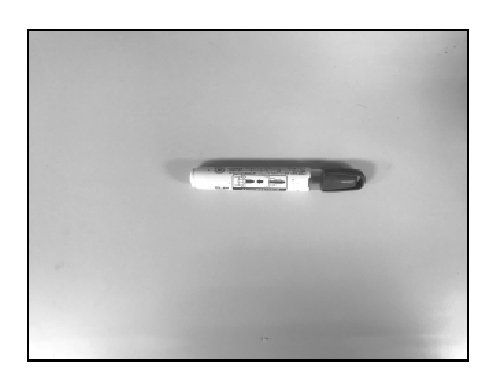
\includegraphics[clip, width=4.5cm]{./figure/pen_glay.eps}
				\hspace{1.6cm} [a] Glay
			\end{center}
		\end{minipage}
		
		% 2
		\begin{minipage}{0.33\hsize}
			\begin{center}
				\includegraphics[clip, width=4.5cm]{./figure/pen_thresh_80.eps}
				\hspace{1.6cm} [b] threshold=80
			\end{center}
		\end{minipage}
		
		% 3
		\begin{minipage}{0.33\hsize}
			\begin{center}
				\includegraphics[clip, width=4.5cm]{./figure/pen_thresh_100.eps}
				\hspace{1.6cm} [c] threshold=100
			\end{center}
		\end{minipage} \\
		
		% 4
		\begin{minipage}{0.33\hsize}
			\begin{center}
				\includegraphics[clip, width=4.5cm]{./figure/pen_thresh_120.eps}
				\hspace{1.6cm} [d] threshold=120
			\end{center}
		\end{minipage} 
		
		% 5
		\begin{minipage}{0.33\hsize}
			\begin{center}
				\includegraphics[clip, width=4.5cm]{./figure/pen_thresh_140.eps}
				\hspace{1.6cm} [e] threshold=140
			\end{center}
		\end{minipage} 
		
		% 6
		\begin{minipage}{0.33\hsize}
			\begin{center}
				\includegraphics[clip, width=4.5cm]{./figure/pen_thresh_160.eps}
				\hspace{1.6cm} [f] threshold=160
			\end{center}
		\end{minipage}

		\end{tabular}
		\caption{単純二値化処理}
		\label{fig:global}
	\end{center}
\end{figure}


本アプリケーションには, 単純閾値処理, Bradlry法, 2つの閾値を用いた閾値処理を実装した. 
%%%%%%%%%%%%%%%%%%%%%%%%%%%%%%%%%%%%
\subsection{Bradley法}
%%%%%%%%%%%%%%%%%%%%%%%%%%%%%%%%%%%%
Bradley法は, 入力画像上の注目画素を中心とする, ある領域内($s \times s$)の画素値の平均値を注目画素の閾値とし, その値が注目画素の画素値よりも$t\%$小さい場合は黒, そうでない場合は白に値を置き換える方法である. すなわち, 注目画素の閾値を式\cite{Center_Thresh}にて計算し,
\begin{equation}
	\label{Center_Thresh}
	S = \frac{1}{N} \sum_{i-\frac{s}{2}}^{i+\frac{s}{2}} \sum_{j-\frac{s}{2}}^{j+\frac{s}{2}} I(i, j)
\end{equation}
その値を基に式\cite{Bradley_Thresh}より, 二値化を行う.
\begin{equation}
	\label{Bradley_Thresh}
	I'(i, j) = \left\{
		\begin{array}{l}
			1 \hspace{4mm} if \hspace{2mm} (I(i, j) \leq S \times \frac{100 - t}{100})\\
			0 \hspace{4mm} otheres
		\end{array}
		\right.
\end{equation}

%%%%%%%%%%%%%%%%%%%%%%%%%%%%%%%%%%%%
\section{2つの閾値を用いた二値化処理}
%%%%%%%%%%%%%%%%%%%%%%%%%%%%%%%%%%%%
この処理は, 単純二値化処理の閾値を2つに増やしたものであり, 

%%%%%%%%%%%%%%%%%%%%%%%%%%%%%%%%%%%%
\section{Canny法を用いたオブジェクト抽出}
%%%%%%%%%%%%%%%%%%%%%%%%%%%%%%%%%%%%
二値画像内において, 物体は画素値が等しいピクセルの集合として表現でき, その重心位置$G(G_x, G_y)$は, 画素値とピクセル座標より式\ref{COG_of_Image}を用いて求めることができる.
\begin{align}
	\begin{aligned}
		\label{COG_of_Image}
		G_x = \frac{\sum_{p=1}^x \sum_{q=1}^y xI(p, q)}{\sum_{p=1}^x \sum_{q=1}^y I(p, q)}\\
		G_y = \frac{\sum_{p=1}^x \sum_{q=1}^y yI(p, q)}{\sum_{p=1}^x \sum_{q=1}^y I(p, q)}
	\end{aligned}
\end{align}
ここで, 画像の原点は左上, $I(p, q)$はあるピクセル座標での画素値である. 
この式はオブジェクトが画像中に1つしかない場合のみ適応可能である. しかし, オブジェクトが1つのみの画像は稀であり, またカメラに付着した埃などにより背景に穴ができた場合も前述の式では, 重心位置がずれてしまう.
そこで, 背景を除き画像内でピクセル集合(面積)が最大のものを目的のオブジェクトであると仮定し, その集合に対してのみ重心位置を求めることにする. 

具体的には, まずラベリング処理により, 背景からオブジェクトを分離し, それぞれの面積を計算する. その後, 面積が最大のものに対して重心位置を計算する. 

ラベリング処理とは, 2値画像上に点在している連結成分のそれぞれに固有の名前(番号など)を付ける処理であり, これにより連結成分の個数やそれぞれの特徴(面積など)を独立して計算可能である. また, 連結成分とは, 図\ref{fig:4conne_and_8conne}に示すように中心画素とその周囲のいくつかの画素が同値で存在する領域を指し, 連結の種類には4連結と8連結がある. 
%------------
%connections
%------------
\begin{figure}[ht]
	\begin{center}
		\includegraphics[width=75mm,clip]{./figure/gazou.eps}
		\caption{4 connections and 8 connections}
		\label{fig:4conne_and_8conne}
	\end{center}
\end{figure}
この2つの連結性のうち, どちらか一方を背景, 他方を検出したい物体に適用することで, 背景とオブジェクトの境界付近にあるピクセルの孔の影響を抑え, それらを分離することができる. 本アプリケーションでは, デフォルトで8連結をオブジェクトに適用している. 

分離された個々のオブジェクトの面積は, それに内包されるピクセル数を数えることで求めることができる. そして, 面積が最も大きい集合の画像全体に対する重心位置$G'(G'_x, G'_y)$は次式で求められる.
\begin{align}
	\begin{aligned}
		\label{COG_of_Image'}
	G'_x = \frac{\sum_{p=1}^x \sum_{q=1}^y xI'(p, q)}{S_{max}}\\
	G'_y = \frac{\sum_{p=1}^x \sum_{q=1}^y yI'(p, q)}{S_{max}}
	\end{aligned}
\end{align}
ここで, $I'$は次の条件を満たす画素値であり, $S_{max}$は面積の最大値である.
\begin{equation}
	I'(i, j) = \left\{
		\begin{array}{l}
			1 \hspace{4mm} if \hspace{2mm} (I(i, j) \in S_{max})\\
			0 \hspace{4mm} others
		\end{array}
		\right.
\end{equation}


%%%%%%%%%%%%%%%%%%%%%%%%%%%%%%%%%%%%%%%%%%%%%%%%%%%%%%%%%%%%%%%%
%%%%%%%%%%%%%%%%%%%%%%%%%%%%%%%%%%%%%%%%%%%%%%%%%%%%%%%%%%%%%%%%
%%%%%%%%%%%%										%%%%%%%%%%%%
%%%%%%%%%%%%				第4章					%%%%%%%%%%%%
%%%%%%%%%%%%										%%%%%%%%%%%%
%%%%%%%%%%%%%%%%%%%%%%%%%%%%%%%%%%%%%%%%%%%%%%%%%%%%%%%%%%%%%%%%
%%%%%%%%%%%%%%%%%%%%%%%%%%%%%%%%%%%%%%%%%%%%%%%%%%%%%%%%%%%%%%%%
%%%%%%%%%%%%%%%%%%%%%%%%%%%%%%%%%%%%%%%%%%%%%%%%%%%%%%%%%%%%%%%%%%%%%%%%%%%%%
\chapter{人工知能}
%%%%%%%%%%%%%%%%%%%%%%%%%%%%%%%%%%%%%%%%%%%%%%%%%%%%%%%%%%%%%%%%%%%%%%%%%%%%%

%%%%%%%%%%%%%%%%%%%%%%%%%%%%%%%%%%%%
\section{人工知能}
%%%%%%%%%%%%%%%%%%%%%%%%%%%%%%%%%%%%
人工知能(AI : Artifical IntelligenceI)は, 「どのようなデータを, どのようなアルゴリズムで処理すれば, 人間のような知能(認識・処理・判断など)を実現することができるのか」について研究する分野であり, 1947年にアラン・チューリングによってその概念が提唱された.

現在のAIに関する技術(AI技術)や応用分野については, 文献\cite{JSAI-2019}が詳しいので, そちらを参照されたい. 
%%%%%%%%%%%%%%%%%%%%%%%%%%%%%%%%%%%%
\section{機械学習}
%%%%%%%%%%%%%%%%%%%%%%%%%%%%%%%%%%%%
機械学習とは, 「ルールの記述が難しい問題(例えば1枚の画像から人の顔を見分ける問題)」に対して, 人間がルールを決めるのではなく, コンピュータ自体にルールを発見させようする手法」である. 機械学習において, コンピュータがルールを発見するまでの過程を「学習」, 発見されたルールをモデルといい,  このモデルを用いて画像や音声などの判定(認識)を行う. 
学習には, 以下の3タイプがありルールの発見方法がそれぞれで異なる.
\begin{itemize}
  \item 教師あり学習
  \item 教師なし学習
  \item 強化学習
\end{itemize}


機械学習の分類は, 文献\cite{Kamishima-2019}が詳しいので, そちらを参照されたい. 
%%%%%%%%%%%%%%%%%%%%%%%%%%%%%%%%%%%%
\section{ニューラルネットワーク}
%%%%%%%%%%%%%%%%%%%%%%%%%%%%%%%%%%%%

%%%%%%%%%%%%%%%%%%%%%%%%%%%%%%%%%%%%
\section{畳み込みネットワーク}
%%%%%%%%%%%%%%%%%%%%%%%%%%%%%%%%%%%%



%%%%%%%%%%%%%%%%%%%%%%%%%%%%%%%%%%%%%%%%%%%%%%%%%%%%%%%%%%%%%%%%
%%%%%%%%%%%%%%%%%%%%%%%%%%%%%%%%%%%%%%%%%%%%%%%%%%%%%%%%%%%%%%%%
%%%%%%%%%%%%										%%%%%%%%%%%%
%%%%%%%%%%%%				第5章					%%%%%%%%%%%%
%%%%%%%%%%%%										%%%%%%%%%%%%
%%%%%%%%%%%%%%%%%%%%%%%%%%%%%%%%%%%%%%%%%%%%%%%%%%%%%%%%%%%%%%%%
%%%%%%%%%%%%%%%%%%%%%%%%%%%%%%%%%%%%%%%%%%%%%%%%%%%%%%%%%%%%%%%%
%%%%%%%%%%%%%%%%%%%%%%%%%%%%%%%%%%%%%%%%%%%%%%%%%%%%%%%%%%%%%%%%%%%%%%%%%%%%%
\chapter{実機による動作実験}
%%%%%%%%%%%%%%%%%%%%%%%%%%%%%%%%%%%%%%%%%%%%%%%%%%%%%%%%%%%%%%%%%%%%%%%%%%%%%

%%%%%%%%%%%%%%%%%%%%%%%%%%%%%%%%%%%%
\section{Dobot}
%%%%%%%%%%%%%%%%%%%%%%%%%%%%%%%%%%%%
TechShare社が販売しているDobot Magician(Dobot)は, 4自由度のロボットアームでありエンドエフェクタを取り換えることによって3Dプリンタのような積載加工, エンドミルによる切削加工ペンツールを使った印字などが行える. 
Dobotの質量と可搬質量はそれぞれ3.4kgと500gであり, 位置繰り返し精度は0.2mmと教育ロボットとしては優れている. 
またDobot社より, CやMFC(Microsoft Foundation Class), Pythonなど複数のプログラミング言語でAPIが提供されており, 個人でプログラムを組む際の敷居も低い. 
今回は, その中のPython APIを統合開発環境であるVisual Studio2019上に実装し, Dobot本体を動作させるプログラムの開発を行った. APIとはあるコンピュータプログラム(ソフトウェア)の機能や管理するデータなどを、外部の他のプログラムから呼び出して利用するための手順やデータ形式などを定めた規約のことである. 
今回はその中からDobot本体の姿勢を取得するためのGetPose()
また, Pythonに標準で搭載されているGUI作成キットであるTkinterを用いて, 開発した動作プログラムを簡単に扱えるようDobot制御用のユーザインタフェースの作成も行った. 

%%%%%%%%%%%%%%%%%%%%%%%%%%%%%%%%%%%%
\section{学習データ}
%%%%%%%%%%%%%%%%%%%%%%%%%%%%%%%%%%%%

%%%%%%%%%%%%%%%%%%%%%%%%%%%%%%%%%%%%
\section{実験結果}
%%%%%%%%%%%%%%%%%%%%%%%%%%%%%%%%%%%%


%%%%%%%%%%%%%%%%%%%%%%%%%%%%%%%%%%%%%%%%%%%%%%%%%%%%%%%%%%%%%%%%
%%%%%%%%%%%%%%%%%%%%%%%%%%%%%%%%%%%%%%%%%%%%%%%%%%%%%%%%%%%%%%%%
%%%%%%%%%%%%										%%%%%%%%%%%%
%%%%%%%%%%%%				第6章					%%%%%%%%%%%%
%%%%%%%%%%%%										%%%%%%%%%%%%
%%%%%%%%%%%%%%%%%%%%%%%%%%%%%%%%%%%%%%%%%%%%%%%%%%%%%%%%%%%%%%%%
%%%%%%%%%%%%%%%%%%%%%%%%%%%%%%%%%%%%%%%%%%%%%%%%%%%%%%%%%%%%%%%%
%%%%%%%%%%%%%%%%%%%%%%%%%%%%%%%%%%%%%%%%%%%%%%%%%%%%%%%%%%%%%%%%%%%%%%%%%%%%%
\chapter{今後の方針}
%%%%%%%%%%%%%%%%%%%%%%%%%%%%%%%%%%%%%%%%%%%%%%%%%%%%%%%%%%%%%%%%%%%%%%%%%%%%%









\backmatter% ここから後付
\chapter{謝辞}%%%%%%%%%%%%%%% 謝辞 %%%%%%%
本研究は,山口東京理科大学大学院基礎工学研究科基礎工学専攻で行われたものである.
\begin{thebibliography}{}%%%参考文献%%%%%%
\bibitem{Iziri-2019}
井尻善久, F. Drigalski, ``産業用ロボットの進化によるものづくりの近未来", 日本ロボット学会誌, Vol. 37, No. 8, pp. 5-8, 2019.

\bibitem{Otsu-1979}
N. Otsu, ``A Threshold Selection Method from Gray-Level Histograms.", IEEE Transactions on Systems. Man. and Cybernetics, Vol. 9, No. 1, pp. 62?66, 1979.

\bibitem{Bradley-2007}
D. Bradley, G. Roth, ``Adapting Thresholding Using the Integral Image", Journal of Graphics Tools, Vol. 12, No. 2, pp.13?21, 2007.

\bibitem{JSAI-2019}
https://www.ai-gakkai.or.jp/resource/aimap/

\bibitem{Kamishima-2019}
神嶌敏弘, 鹿島久嗣, ``機械学習分野の俯瞰と展望'', 人工知能学会誌, Vol. 34, No. 6, pp. 905-915, 2019.

\end{thebibliography}
\end{document}